% set document class
\documentclass[a4paper,notitlepage,12pt]{article}

% load packages
\usepackage[utf8]{inputenc}
\usepackage[english]{babel}
\usepackage[a4paper, margin=0.8in]{geometry}
\usepackage{graphicx}
\usepackage{amsmath}
\usepackage{authblk}
\usepackage{hyperref}
\usepackage[backend=biber,style=nature]{biblatex}

% specify bibliography source
\addbibresource{main.bib}
\renewcommand*{\bibfont}{\small}

% specify link style
\hypersetup{
    colorlinks=true,
    linkcolor=blue,
    filecolor=magenta,      
    urlcolor=cyan,
    citecolor=blue
}

% specify some custom commands
\renewcommand{\baselinestretch}{1.2}
\renewcommand*{\Authsep}{, }
\renewcommand*{\Authand}{, }
\renewcommand*{\Authands}{, }
\renewcommand*{\Affilfont}{\normalsize}

% set up the author block
\setlength{\affilsep}{2em}   % set the space between author and affiliation
\author[1]{Samuel Zorowitz}
\author[1,2]{Yael Niv}
\affil[1]{Princeton Neuroscience Institute, Princeton University, USA}
\affil[2]{Department of Psychology, Princeton University, USA}

% specify the title
\title{Improving the reliability of cognitive task measures: A narrative review}

% turn date off
\date{}

% Define paragraph formatting
\setlength{\parindent}{0em}
\setlength{\parskip}{1em}

\begin{document}

\maketitle

\section{Introduction}

% P1: Using valid and reliable measures of behavior is crucial for advancing biological psychiatry.

Cognitive tasks have already demonstrated, and continue to hold, tremendous promise for biological psychiatry. Variability in performance on cognitive tasks provides experimenters with crucial insights into the relationship between individual differences in cognitive processing and behavioral phenomena outside of the laboratory or clinic (e.g. reward sensitivity in a monetary-incentivized task and anhedonia in depression). Elsewhere in psychology, cognitive tasks have been useful in predicting important outcomes such as academic achievement \cite{spiegel2021relations} and cognitive decline \cite{hartshorne2015does}. Cognitive tasks, then, are invaluable tools for building and refining our understanding of psychiatric symptoms and syndromes. For a cognitive task to be useful in this regard, however, it must possess sufficient measurement properties. 

% P2: Definitions + Three key properties of behavioral measures: discriminability, reliability, and validity

We define a cognitive task as any experimental paradigm that measures behavior in order to make inferences about one or more cognitive processes (e.g. Stroop task, delay discounting task, reversal learning task). Cognitive-task measures for characterizing individual differences are descriptive or model-based indicators of behavioral performance such as proportion correct, average response time, and learning rate. The psychometric quality of such a measure can be summarized by three key properties: \emph{discriminating power}, \emph{validity} and \emph{reliability} \cite{kline2015handbook}. The discriminatory power of a task measure describes its ability to measure variability in participants' performance. This is a necessary property of tasks to be used for studying individual differences; where there is no variation in performance, there are no individual differences to study. The validity of a task measure concerns whether it actually measures what it purports to measure. Finally, the reliability of a task measure characterizes the degree to which it consistently rank-orders participants across measurement instances. Put another way, a task measure is reliable if, assuming participants have not changed, it produces the same score for each participant over time. The focus of this review is task reliability, which is a prerequisite for validity. 

% P3: definition and Importance of reliability
\subsubsection*{The formal definition of reliability}

In classical test theory, the variance in observed scores on a task measure $X$ is the sum of the true score variance $T$, reflecting real individual differences in the latent construct of interest, and measurement error $E$, i.e., $X = T + E$. The reliability of a measure is defined as the proportion of variance attributable to the true score variance relative to total variance: $\rho = \frac{T}{T + E}$. Thus, reliability quantifies the magnitude of individual differences relative to the noisiness of a task measure; the larger the reliability of a task measure, the more it reflects true individual differences rather than reflecting noise. Reliability is therefore a prerequisite for validity: an unreliable task measure reflects measurement error and not the construct of interest. If this were not reason enough to care about reliability, the observed correlation between two measures (e.g. task performance and self-reported symptom score) is bounded by their individual reliabilities \cite{Spearman1904-mo}: 
\begin{equation}
    \rho_{xy} = \rho_{tt} \sqrt{\rho_{xx'} \cdot \rho_{yy'}}
\end{equation}
where $\rho_{xx'}$ and $\rho_{yy'}$ are the reliabilities of two measures, $x$ and $y$; $\rho_{tt}$ is their true latent correlation; and  $\rho_{xy}$ is their observed correlation. As all reliabilities are $<1$, the reliability of a measure places an upper bound on the maximum observable correlation between itself and a second measure (Figure \ref{fig:fig01}). As an important corollary, as measure reliability decreases, the number of participants required to reliably detect a correlation between two measures increases \cite{Parsons2019-jw}. Thus, poor reliability hampers our ability to investigate associations between cognitive processes, as measured by task performance, and other variables of interest. 

\begin{figure}[tp]
    \centering
    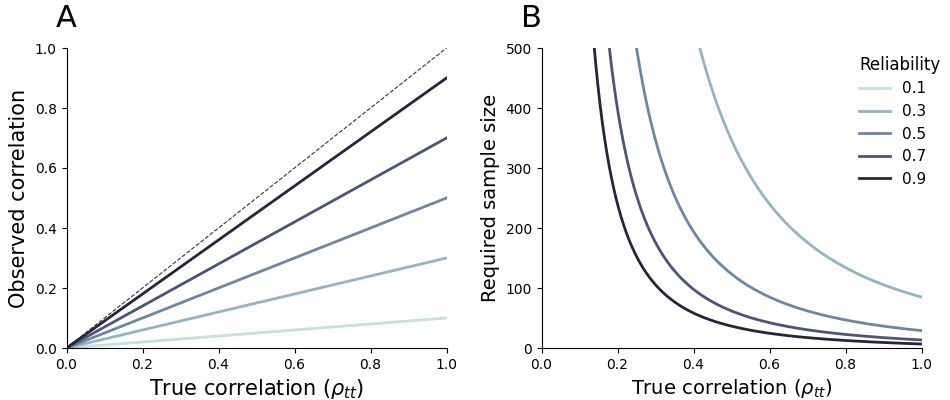
\includegraphics[width=1.0\textwidth]{figures/fig01.png}
    \caption{\small The relationship between measure reliability, observed correlations, and statistical power. (A) The maximum expected observed correlation between two measures as a function of their true (latent) correlation and reliability. As the reliability of two measures decreases, so too does their observed correlation. (B) Required sample size for 80\% power to detect true correlations between two measures given their reliability. As the reliability of two measures decreases, the number of participants required to detect an association increases. Even with a large sample size of $N=500$, a measure with reliability $\rho_{tt} = 0.5$ will only allow detection of correlations above $0.3$, which are uncharacteristically high in the field.}
    \label{fig:fig01}
\end{figure}

% P4: Reliability is inherently context-dependent: it is a function of the population, task, and testing context

To further complicate matters, the reliability of a task measure is not absolute -- it reflects interactions between task design, the participants, and the context in which the task is administered. Indeed, task reliability can vary as a function of parameters of the experiment such as the specific stimulus set, number of trials, time limits \cite{paap2016role, cooper2017role}); sample populations (healthy adults, children, psychiatric patients \cite{arnon2020current, cooper2017role}); testing locations (in clinic, online); response modality (desktop, smartphone, virtual reality \cite{pronk2022can, bruder2021reliability}); and scoring or estimation method \cite{Rouder2019-am, haines2020learning}. For example, a cognitive task originally designed for use with an adult population may prove too difficult for children. Their task performance may drop to chance level, thereby minimizing between-participant variance and, as a consequence, task reliability. As a second example, participants completing an experiment online from their homes may experience more distraction than if they participated in the lab. This may increase the measurement error, leading to a concomitant decrease in reliability. Experimenters therefore cannot assume the reliability of a task measure is constant. Ideally researchers would investigate and report the reliability of task measures as part of any analysis or, at the very least, after having made changes to a task or scoring procedure or when administering the task to new sample populations or in new testing contexts.

% P5: Task reliability lower on average

Although verifying the reliability of cognitive task measures is paramount to individual-differences research, the reliability of task measures is seldom reported \cite{Green2016-xw, Parsons2019-jw}. When they are reported, task measures frequently exhibit lower reliability than what is conventionally considered acceptable for individual-differences research ($\rho_{tt}$ on the order of 0.7 - 0.8) and the reliability regularly achieved by self-report measures. Indeed, many studies have now found that task measures exhibit moderate-to-low reliability \cite{Hedge2018-lf, Frey2017-uz, Enkavi2019-oh, Von_Bastian2020-tm, Nitsch2022-pe, verdejo2021unified}.

One possible explanation for this finding is the so-called ``reliability paradox'' of cognitive tasks \cite{Hedge2018-lf}, which states that the often lackluster reliability of tasks is a result of a mismatch in goals between experimental and individual-differences psychological research. In experimental psychology, the goal is often to demonstrate the existence of a behavioral effect. One means of increasing the power to detect an effect is to minimize between-participants variance. This is the exact opposite of what is desirable for individual differences research, where between-participants variance is essential to achieving reliable task measures. Thus, the tendency in biological psychiatry to adopt the most prominent tasks in experimental psychology---the ones that most reliably demonstrate a behavioral effect---may actually hamstring our efforts to study individual differences. 

% P6: Purpose of paper: narrative review of task reliability

Regardless, we do not believe that task measures are inherently less reliable than self-report measures, and that pessimism about task-based individual-differences research is warranted. It is possible to (re)design tasks to achieve good reliability, even to the high levels dictated by conventional standards \cite{waltmann2022sufficient, sullivan2022enhancing, kucina2022solution, snijder2022psychometric}. The purpose of the current article is to provide a narrative review of approaches to improve task-measure reliability. The article is divided into two main parts. First, we review methods of calculating reliability and discuss some nuances that are specific to cognitive tasks. Then, we introduce a taxonomy of approaches for improving task reliability using concrete examples from the published literature. We hope that this article can serve as a helpful guide for experimenters who wish to design a new task, or improve an existing task, to achieve sufficient reliability for use in individual-differences research.

\section{Calculating reliability}

There are two measures of reliability of relevance for task measures: internal consistency and test-retest reliability. Internal consistency is the reliability of a measure in a single administration of a task. Test-retest reliability (also known as temporal stability) is the reliability of a task measure across two or more administrations. Even for cross-sectional experiments, where stability over time is of no scientific interest, test-retest reliability is a useful index. This is because estimates of internal consistency tend to be inflated due to between-participants variance from construct-irrelevant, state-dependent factors (e.g. current mood, fatigue). Given sufficient time between testing sessions, test-retest reliability should be less biased by state factors, and thus a better estimate of the true cross-sectional task-measure reliability. However, whereas high internal consistency is always desirable for individual difference studies, high test-retest reliability may not be, depending on the construct a researcher is intending to measure. Low one-month test-retest reliability may not be problematic for an index of a transient cognitive process (e.g., mood-dependent attentional biases), but is a problem if individual differences in a cognitive process are hypothesized to be stable across time (e.g., extraversion and social reward processing).

The test-retest reliability of a task measure can be calculated in numerous ways \cite{Parsons2019-jw}. Perhaps the simplest approach is to compute the Pearson correlation between participants' scores from two sessions. An alternative approach is to calculate the intraclass correlation coefficient (ICC), which decomposes a task measure into true score variance and error variance. There are many formulas for calculating ICC \cite{Koo2016-fz}, with the critical distinction being whether reliability is based on the \textit{consistency} or \textit{absolutely agreement} of a task measure across two administrations. Consistency-based ICCs are affected only by the relative ordering of participants across time; that is, they are insensitive to systematic changes to the actual values of a task measure across time (e.g., due to practice effects on task performance). In contrast, absolute-agreement based ICCs measure the degree to which scores are stable across time. The type of ICC to use depends on the experimenter's goals and the ultimate use of the task measure. % desiderata from the measured individual differences. %If an experimenter cares only about the rank-ordering of participants across time, a consistency-based ICC (or Pearson correlation) is preferable. Conversely, if systematic differences in a task measure across task administrations is a concern, then an absolute agreement-based ICC should be preferred. 

Calculating the internal consistency of a task measure is more complicated. The most common measure of internal consistency, Cronbach's $\alpha$, requires certain assumptions that are unrealistic for many task data (e.g., equivalence of trials, uncorrelated measurement error). As such, internal consistency for task measures is instead usually calculated via split-$K$ reliability, where $K$ indicates the number of splits. Split-half reliability ($K=2$) is most common. A critical challenge in calculating split-half reliability is in deciding how to partition the data, as estimates of reliability may be biased when partitions are not equally good measures of a behavior \cite{Green2016-xw, pronk2022can}. For example, first-second splitting (i.e., partitioning the data into the first and second halves of an experiment) may underestimate reliability due to differences between the partitions due to practice, fatigue, or other linear time effects. In contrast, odd-even splitting (i.e., partitioning the data into odd and even trials) may be confounded when behavior across trials is non-independent (i.e., measurement error is correlated across trials). Under such conditions, odd-even splitting will artificially inflate the similarity of data across partitions, thereby decreasing estimates of measurement noise and overestimating reliability. Therefore, where possible, a permutation-based approach to calculating split-half reliability is recommended \cite{pronk2022can, Parsons2019-jw}. Here, reliability is averaged across many thousands of random partitions of the data into halves. For task measures derived from cognitive models, however, it may be prohibitively computationally intensive to employ such an approach due to the need to re-estimate the task measure for each new subset of the data. Moreover, for learning tasks that are commonly used in computational psychiatry, cognitive model-based task measures cannot be estimated from only a subset of the trials due to inherent non-independence of task behavior across trials. In these cases, one can design tasks with at least two independent blocks. Then a model is fit to each block independently and reliability is calculated using the model parameters estimated from each. 

As a final point, traditional sum or mean score estimates of performance (e.g., proportion correct responses, mean response time) may substantially underestimate task reliability in cases where some response variability across trials can be accounted for rather than treated as noise \cite{Rouder2019-am, haines2020learning}. These summary scores are noisy (and thus less reliable) estimates of task performance as they neglect trial-by-trial variability. Instead, it is often preferable to use generative or statistical models that account for trial-level variability in behavior. By directly modeling trial-by-trial variability, estimates of participants' performance are effectively de-noised. It is also advisable to use hierarchical models that partially pool data across participants, which in turn further increases the precision of estimates of participants' performance. Together, these methods can substantially boost estimates of reliability \cite{Rouder2019-am, haines2020learning}, as multiple studies have demonstrated  \cite{snijder2022psychometric, sullivan2022enhancing, brown2020improving, waltmann2022sufficient}. For a detailed discussion of generative models in the context of task reliability, see Haines (this issue).

\section{Improving task reliability}

As defined above, the reliability of a task measure is the proportion of variance attributable to between-participant differences relative to measurement error. Thus, the two major strategies for improving the reliability of a measure are to increase between-participant variability or decrease measurement error. In what follows, we discuss approaches for accomplishing each objective in turn. Where appropriate, we highlight studies that are exemplary for improving the reliability of a task measure by implementing a particular strategy. 

\subsection{Increasing between-participant variance}

\subsubsection{Ceiling \& floor effects}

By definition, the reliability of a task measure is zero when there is no variability across participants. Thus, range restriction of task measures via ceiling or floor effects is a serious obstacle to reliability. Siegelman and colleagues \cite{siegelman2017measuring} noted the consequences of floor effects on reliability in the context of statistical learning tasks. In such tasks, participants must learn to identify subtle patterns in the transition probabilities underlying a continuous sequence of stimuli. In reanalyzing archival datasets, Siegelman and colleagues found a majority of participants were at chance-level performance in discriminating between legitimate and foil sequence patterns; consequently, the reliability of conventional proportion correct measures suffered. In response, the authors designed a new statistical learning task involving stimulus sequences that ranged more widely in their difficulty to learn. Only a minority of participants showed chance-level performance on this new task and, as such, the reliability of proportion correct scores improved. Similarly, in developing an abbreviated working-memory task, Oswald and colleagues \cite{oswald2015development} found that they could remove the easiest trials---those with ceiling level performance---with virtually no change to task reliability. This is because those trials are incapable of differentiating ability across participants and therefore cannot contribute significantly to the reliability of the task.

Researchers administering a task to a new population should be especially wary of range-restriction effects. Cognitive tasks calibrated for one group of participants may not be adequately sensitive for others due to being too easy or difficult for a different group. For example, Arnon and colleagues \cite{arnon2020current} found that statistical learning tasks developed for adults were too difficult for young children and therefore yielded unreliable discrimination scores in that population. Similarly, Kyllonen and colleagues \cite{kyllonen2019general} were motivated to develop a battery of fluid-reasoning measures for highly educated adults due to observed ceiling effects in performance when using preexisting fluid-reasoning tasks in this population.  

\subsubsection{Repeatability \& practice effects}

A related issue for task reliability is practice effects, where participants' performance on a task improves with repeated administrations. Practice effects are relatively common for cognitive tasks \cite{hausknecht2007retesting, scharfen2018retest}. They might occur due to the attenuation of task-irrelevant nuisance factors (e.g. performance anxiety) and/or the learning of task-specific knowledge or strategies. Practice effects are not inherently an issue for reliability --- especially if an experimenter is only interested in the consistency, but not the absolute agreement, of participants' performance over time --- but they can become a pernicious issue if they are severe enough to induce ceiling effects. For example, Paredes and colleagues \cite{paredes2021psychometric} observed large practice effects on the Pavlovian go/no-go task for short retest intervals (3 days, 14 days), which resulted in poor estimates of test-retest reliability. In developmental and lifespan studies, practice effects are potentially complicated by their interaction with age \cite{anokhin2022age, salthouse2010influence}; that is, practice-induced ceiling effects may present in some age groups but not others. 

One strategy for minimizing practice effects is simply to increase the time interval between task administrations. The more time that elapses between sessions, the greater the probability that participants will have forgotten task-specific knowledge or strategies \cite{hausknecht2007retesting, scharfen2018retest}. Of course, this solution may not always be possible or desirable, especially if a researcher is only able to or specifically interested in studying a behavior over a short time period. Moreover, some forms of learning do not easily dissipate with time.

A second strategy is to design tasks so as to prevent or discourage the formation of task-specific strategies. For example, McLean and colleagues \cite{mclean2018towards} investigated the repeatability of the beads task. In the beads task, participants are presented with two jars containing beads of two colors in equal but opposite ratios. In each trial of the task, a predetermined sequence of beads is drawn from one jar. Participants must decide which jar beads were being drawn from or request to see more beads. In a typical version of the task, the same sequence of bead draws is used across all trials. McLean and colleagues found that participants were aware that the sequence repeated across trials and, as a consequence, became more erratic in their decision to witness more bead draws with additional trials. In response, the authors developed a new version of the task that included distractor sequences of bead draws. This new design was effective in preventing participants from becoming aware of the target sequence, which in turn resulted in more consistent responding, which improved the reliability of participants' information seeking scores. 

\subsubsection{Enhancing experimental effects}

The preceding sections described potential threats to between-participants variability, but not approaches to improve it. A primary strategy for increasing between-participants variability is to enhance the experimental effect. Amplifying the magnitude of an experimental effect (e.g., making a task more challenging, increasing the potency of affect induction) typically increases the range of participants' responses to it. For example, Kucina and colleagues \cite{kucina2022solution} investigated the reliability of cognitive conflict effects in new versions of several standard cognitive-control tasks (e.g., Stroop, Flanker, Simon) that amplified cognitive interference via two task design features. First, they combined multiple sources of cognitive interference in the same task, for example by combining the Stroop and Simon effects to create a ``Stroopon'' task. Second, for a subset of trials, they required participants to make multiple responses based on both relevant and irrelevant stimuli attributes. Compared to the standard version of these tasks, these experimental manipulations had the effect of increasing task demands, which resulted in greater between-participants variance, and higher reliability as a consequence. (See also Snijder and colleagues \cite{snijder2022psychometric} for a similar redesign of classic cognitive-control tasks that improved reliability by increasing proactive control demands.)

% Similarly, Snijder and colleagues \cite{snijder2022psychometric} studied the reliability of cognitive conflict effects in multiple redesigned cognitive-control tasks (e.g., Stroop, AX-CPT, Cued Task Switching, Sternberg) that required of participants either more proactive control (i.e., maintained vigilance) or more reactive control than the traditional versions of these tasks. The authors found that the proactive control versions of the task were more demanding, which similarly led to larger cognitive interference effects and better task reliability. 

A related strategy is to calibrate the difficulty of the task to the average ability of the population of interest. For example, consider a task trial with two response options. Given the Bernoulli distribution, the variance in responses on this trial will be maximal when the probability of choosing either response is equal. Thus, aggregating across many trials, between-participants variance is maximized --- and task reliability is improved --- when the difficulty of all items is matched to the average ability of the sample \cite{gulliksen1945relation, ferrando2007external} (or slightly higher if participants can guess the correct response \cite{lord1952relation, feldt1993relationship}). Of course, this design principle is only helpful to the degree that a researcher knows the average ability level of their participants. If this is unknown or poorly characterized, then it is instead desirable to design a task with trials spanning a uniform range of difficulty. 

\subsubsection{Sample population}

A final strategy for increasing between-participant variance is to simply recruit more diverse samples. While convenient, undergraduate students from a single university are likely to be relatively homogeneous in their cognitive profiles. It may be worthwhile instead to recruit participants from the community or from an online labor market (e.g., Amazon Mechanical Turk, Prolific Academic, CloudResearch Panels). With regard to the latter, because online participants typically complete experiments from their homes or other poorly-controlled environments, they are more likely to be distracted or to multi-task during an experiment \cite{newman2021data}. Thus, when recruiting online samples, experimenters should take special care to ensure that an increase in between-participants variance is not offset by a concomitant increase in measurement noise.

\subsection{Decreasing measurement noise}

\subsubsection{Increasing trial numbers}

Perhaps the most straightforward approach to decreasing measurement error, and thereby increasing reliability, is to increase the number of task trials. In generalizability theory, the relationship between reliability and the number of trials defined as:
\begin{equation}
    \rho = \frac{\sigma^2_T}{\sigma^2_T + \frac{\sigma^2_E}{n}}
\end{equation}
where $\sigma^2_T$ is the true between-participants variance, $\sigma^2_E$ is measurement error (i.e. trial-level variance), and $n$ is the number of trials. In practice, this relationship often holds (e.g. \cite{paap2016role, cooper2017role}) with some exceptions \cite{price2015empirical, klingelhoefer2022robust}. Notably, increasing the number of task trials only benefits reliability if measurement error is random. If increasing task length results in participant fatigue or boredom, measurement noise may systematically increase and reliability will suffer. Increasing the number of trials may be impractical for other reasons, and because of diminishing marginal improvements for reliability, achieving a desired level of reliability through this means alone may require prohibitively long experiments.

\subsubsection{Improving experiment designs}

Measurement error can be reduced through improving the design of experiments, which can be accomplished in many ways. The reliability of a task measure can be improved by including in an experiment only the most discriminating stimuli. For example, in the context of an emotion recognition task, stimuli of good discriminability would be those where participants with good emotion-recognition ability consistently correctly identify the displayed emotion while participants with poor ability consistently incorrectly identify the displayed emotion \cite{keutmann2015generating}. In contrast, stimuli with poor discriminability --- those for which performance between high- and low-ability participants is indistinguishable --- will lead to more measurement noise and decreased reliability. In experiments where stimuli are intended to be unique and distinguishable, improving both the linguistic and visual distinctness of stimuli may prevent confusion and therefore aid reliability \cite{yoo2022importance}.  

Other design features of an experiment that are specific to the task mechanics may affect reliability. Consider for example the dot-probe task, in which participants must disengage attention from a distracting image on one part of the screen in order to identify and respond to the orientation of a pair of dots elsewhere on the screen. Dot-bottom trials, where a participant must disengage from a distracting stimulus located at the top of the screen and saccade to the bottom of the screen, are more reliable than dot-top trials \cite{price2015empirical, aday2019extended}. This has been explained by suggesting that participants are biased to gaze towards the top of the screen, thus saccading away from the top of the screen requires a stronger level of disengagement, allowing such trials to better measure attentional bias. 

It is worth stressing that clear instructions are essential for task reliability. When participants are unsure of what they are intended to do in an experiment, their behavior is likely to be more variable across time (as their understanding of the task evolves) and across participants (due to different interpretation of instructions), thereby diminishing reliability. (Clear instructions may also work to ensure the validity of an experiment by discouraging participants from using strategies not of interest to the experimenter.) In their ``10 simple rules'' paper for designing cognitive experiments \cite{barbosa2022practical}, Barbosa and colleagues provide practical suggestions for writing task instructions. When adapting a task for a new population, experimenters should ensure that the instructions are still appropriate. Task instructions that are comprehensible to healthy adult participants may not be suitable for other populations like children \cite{hughes2002measuring}. 

Another strategy to reduce measurement error is to make use of a practice phase. Practice trials can help to minimize the effects of nuisance factors such as performance anxiety or unfamiliarity with the response modality, and give participants an opportunity to make sure they understand the task instructions. Thus, practice trials can help participants reach a ``steady state'' of responding, thereby reducing the noisiness of their responses across task trials and increasing reliability \cite{alexander2003effects}. Practice can take the form of a standalone practice block or by designating as such and discarding (or modeling separately) the first few trials of an experiment \cite{mclean2018towards}, though the latter may not fully allow participants to explore response options during the practice. 

Yet another strategy to diminish measurement error is to ``gamify'' an experiment. Incorporating (video) game design elements into cognitive tasks can increase participant engagement and motivation \cite{sailer2017gamification}, countering the would-be effects of boredom and fatigue on task reliability. For example, Kucina and colleagues \cite{kucina2022solution} cite task gamification as an important factor that contributed to the improved the reliability of their cognitive-control tasks. Similarly, Verdejo and colleagues \cite{verdejo2021unified} partially attribute the improved reliability of their impulsivity task battery to gamified task design. 

\subsubsection{Reducing parameter estimation noise}

When parameters from cognitive models are used as indices of participants' task performance, another means to improve measure reliability is to decrease estimation noise. The estimation noise of a parameter given an experiment and model can be quantified through simulation \cite{wilson2019ten, palminteri2017importance}. Here, an experimenter generates artificial data for the experiment using representative model parameters and then attempts to recover the model parameters by fitting the model to the simulated data. Estimation noise is the inverse of the (relative or absolute) agreement between the true and recovered parameters. Alterations to experimental design can improve parameter recovery and estimation noise, and multiple frameworks have been proposed for testing and improving experimental designs to aid parameter recovery \cite{broomell2014parameter, melinscak2020computational}. Parameter recovery can also be affected by the model estimation method \cite{Lerche2017-yg, waltmann2022sufficient}. In particular, the partial pooling properties of hierarchical Bayesian models can be especially beneficial for improving parameter recovery and decreasing estimation noise \cite{katahira2016hierarchical}.

A related approach is to use adaptive experimental designs \cite{myung2013tutorial}, where the trials of an experiment are designed in real time so as to present each participant with stimuli or trial types that are matched to their particular response patterns or ability levels. Though undoubtedly a more complex experimental design, adaptive experiments have the advantage of selecting the most informative trials for resolving the ability or preference level of a participant (e.g. as measured by a cognitive model). Adaptive designs have been successfully used in cognitive research, for example to study working memory \cite{gonthier2018measuring} and delay discounting \cite{ahn2020rapid}. For a detailed discussion of adaptive-design experiments, see Ahn (this issue). 

Parameter estimation may be further improved by leveraging additional information. For example, latent variables may be more accurately measured through the inclusion of demographic variables or other covariates \cite{Curran2016-bt} that, if associated to model parameters, can aid in resolving parameter estimates. An extension of this idea is to utilize joint modeling of dependent variables; that is, to design models where multiple observed trial-level variables are predicted simultaneously. For example, the joint modeling of choice and response time has been found to improve the precision and reliability of estimated parameters in cognitive ability testing \cite{bertling2018using} and reinforcement learning \cite{ballard2019joint, shahar2019improving}. It is also possible to incorporate physiological and/or neural correlates of behavior, such as skin conductance response, fMRI BOLD signal, and EEG \cite{palestro2018tutorial}. 

\subsection{Difference scores}

Difference scores deserve special treatment in the context of reliability. Difference scores subtract a measure of a participant's performance in one condition from their performance in another. An example is the classic Stroop interference effect: the average reaction-time difference between congruent and incongruent trials. Difference scores are commonly used because they allow experimenters to isolate particular cognitive processes (e.g. processing cognitive conflict) while controlling for other sources of variance (e.g. perceptual processing, motor ability) through the subtraction of conditions that share that variance. The challenge is that the reliability of a difference score is a function of the reliability of each of its components and the correlation between the components:
\begin{equation}
    \rho_{dd'} = \frac{\sigma^2_x \rho_{xx'} + \sigma^2_y \rho_{yy'} - 2 \rho_{xy} \sigma_x \sigma_y}{\sigma^2_x + \sigma^2_y - 2 \rho_{xy} \sigma_x \sigma_y}
\end{equation}
where $\sigma^2_x$ and $\sigma^2_y$ are the variances of task measures \textit{x} and \textit{y}, $\rho_{xx'}$ and $\rho_{yy'}$ are the reliabilities of task measures \textit{x} and \textit{y}, and $\rho_{xy}$ is the correlation between task measures \textit{x} and \textit{y} \cite{chiou1996reliability}. When the variances of the two measures are equal, this reduces to: 
\begin{equation}
    \rho_{dd'} = \frac{\rho_{xx'} + \rho_{yy'} - 2 \rho_{xy}}{2 - 2 \rho_{xy}}
\end{equation}
From the above equation, one can see that the reliability of a difference score measure is diminished to the extent that its components are correlated. Two measures derived from the same task will often be correlated due to shared domain-general cognitive processes. Thus, it will often (if not always) be the case that difference scores derived from task measures will be less reliable than the average reliability of their components. 

\subsubsection{Enhance \& purify task measures}

The equations above suggest three steps experimenters can take to improve the reliability of difference scores: (1) improve the reliability of the component measures, (2) increase the difference in the magnitude of the variances of the two task measures, and (3) minimize the correlation between the task measures. The first strategy has been our focus so far. The second approach deserves further comment. As discussed elsewhere \cite{chiou1996reliability}, the reliability of a difference score measure increases as the difference between (or the ratio of) the variances of the component measures increases. The intuitive explanation for why this is the case is that, as the variance of one (but not the other) component grows, so to does the proportion of unshared reliable variance. Figure \ref{fig:fig03} shows that even when the correlation of two measures is large, it is possible to achieve acceptable reliability insofar as the variance ratio (i.e. $\sigma_x / \sigma_y$) is high. This speaks to another advantage of increasing the between-participants variability of a measure (insofar that there is an increase in one, but not the other, measure). This fact may help explain the improved reliability of the difference score measures studied by Kucina and colleagues \cite{kucina2022solution}.

\begin{figure}[tp]
    \centering
    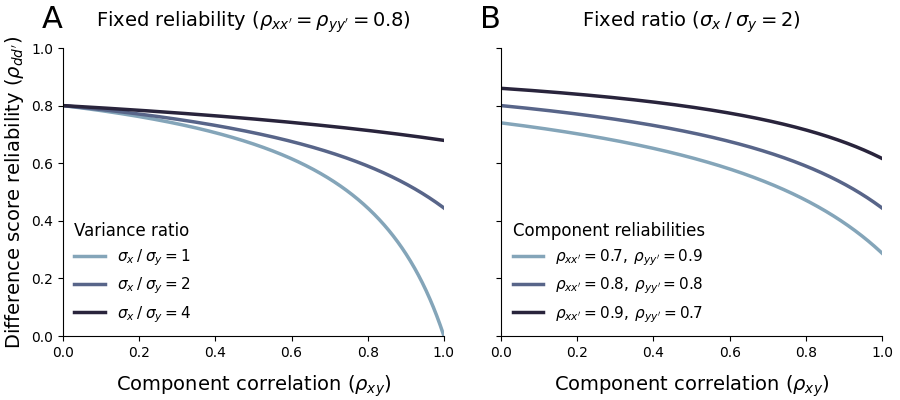
\includegraphics[width=1\textwidth]{figures/fig02.png}
    \caption{Difference score reliability as a function of the variances and reliabilities of its component measures. (A) When the variances of the component measures are equal ($\sigma_x / \sigma_y = 1$), larger correlations between the measures substantially diminish the reliability of a difference score measure. (B) When the variances of the component measures are unequal (e.g., here, $\sigma_x / \sigma_y = 4$), even large correlations between the measures impact the reliability of a difference score measure only minimally. Here, the reliabilities of the component measures are assumed to be equal.}
    \label{fig:fig03}
\end{figure}

The third approach is to purify task measures; that is, to decorrelate the components of a difference score by reducing or eliminating their shared variance. Rey-Mermet and colleagues \cite{rey2019executive} provide an interesting example in the context of executive control. In typical executive control tasks, response times on congruent and incongruent trials are highly correlated, reflecting shared variance from conflict-irrelevant processes including baseline processing speed (e.g. perceptual processing, motor speed) and performance strategies (e.g. individual differences in speed-accuracy preferences; \cite{draheim2019reaction}). Rey-Mermet and colleagues designed a number of ``response-deadline'' executive control tasks where participants had a limited amount of time to respond during a trial. The duration of the response deadline was calibrated for each participant individually such that they achieve a fixed accuracy level in blocks of neutral trials, and  then used as the deadline for both congruent and incongruent trials. The calibration procedure controls for individual differences in processing speed that contribute to performance in both congruent and incongruent trials. It also controls for individual differences in strategy, as regardless of whether a participant was biased towards speed or accuracy, inefficient executive control would result in lower accuracy. With this calibration procedure, the researchers found that the reliability of an accuracy difference score (incongruent - congruent) was as good or better than what had previously been reported for executive control tasks. Thus, controlling for shared variance across measures---that is, purifying measures---can help to improve task reliability.

\subsubsection{Identify alternative measures}

Rather than improving the reliability of difference scores, one can simply avoid using them in the first place. This recommendation has a long history in experimental psychology. Indeed, because difference scores will virtually always be less reliable, many authors have advocated to abandon them \cite{lord1956measurement, cronbach1970we, edwards2001ten}. 

What then are the alternatives to difference scores? Draheim and colleagues \cite{draheim2019reaction} provide an in-depth review of alternatives to difference scores in the context of response-time measures, though much of their discussion is applicable to difference scores in general. One possibility is to simply use the component measures (e.g. performance on incongruent trials in a Stroop task alone). Of course, because component scores will be contaminated other sources of variance, such as baseline performance, interpreting component scores should be done with caution. Another approach is to identify alternative measures of task performance. For example, intra-individual response time variability has been identified as a correlate of executive control that can be measured reliably \cite{saville2011stability} and is altered in psychopathology \cite{kofler2013reaction}. 

\section{Discussion}

% outline
% 1) summarize
% 2) validity: three examples, (1) cognitive control + convergent validity, (2) interpretability of task parameters, (3) predictive validity of tasks (impulsivity), (4) ecological validity. maybe even start with rouder paper: some tasks may not be able to made reliable! other challenges of scaling up, repeated testing, naturalistic contexts (cite germine)
% 3) conclusion: pessimism not warranted. requirements: measuring reliability, sharing case studies for improvement, sharing task code (jspsych-demos)

% inspiration 
% The findings presented here convey the importance of scrutinizing the psychometric properties of cognitive tasks, especially those intended for use in individual differences studies. Reliability is not always reported or even examined by researchers, and the present results also demonstrate why variability and reliability should be considered and reported in the context of one another. Future research efforts related to individual differences in cognition could benefit from incorporating psychometric techniques. This may hopefully lead to improvements in the design and evaluation of cognitive tasks for the purposes of individual differences research.

\printbibliography

\end{document}
